\section{Evaluation}

\begin{table*}[t!]
    \vspace{-0.5in}
    \centering
    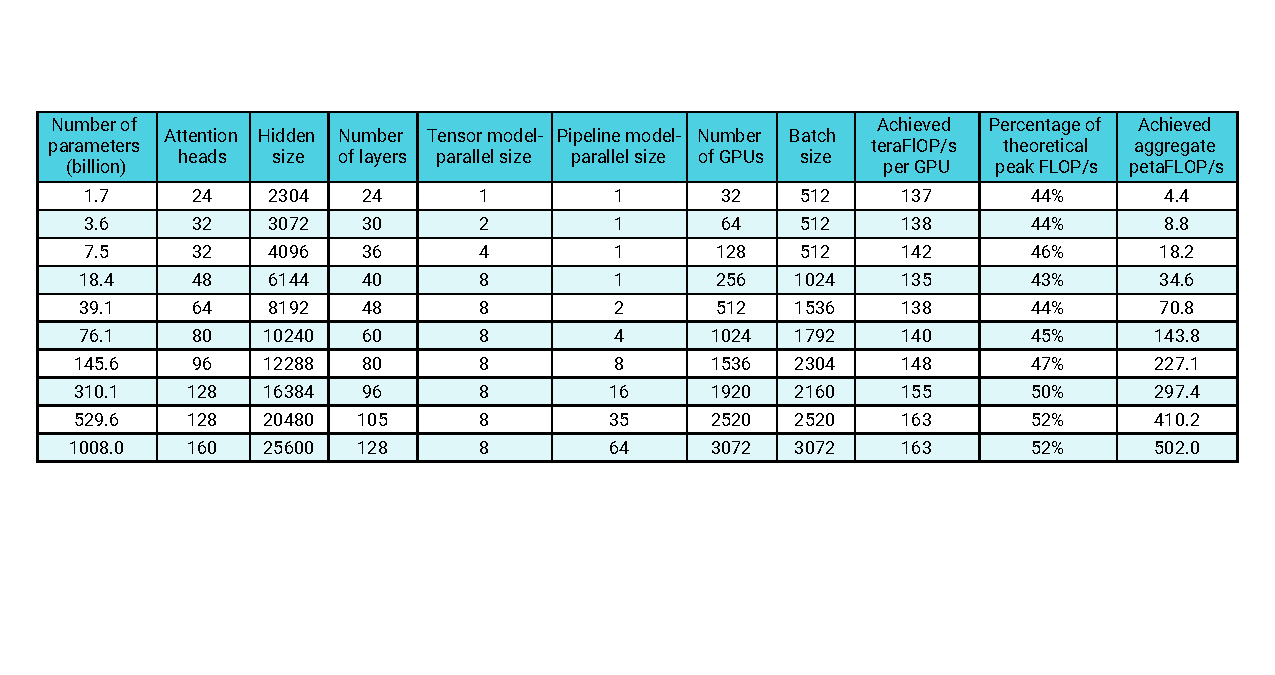
\includegraphics[keepaspectratio=1.0,width=0.97\textwidth]{figures/megatron_scaling_v2.pdf}
    \vspace{-1.1in}
    \caption{
         Weak-scaling throughput for GPT models ranging from 1 billion to 1 trillion parameters.
    }
    \label{fig:megatron_scaling}
    \vspace{-0.3in}
\end{table*}

In this section, we seek to answer the following questions:
\begin{itemize}
    \item How well does PTD-P perform? Does it result in realistic end-to-end training times?
    \item How well does pipeline parallelism scale for a given model and batch size? How much impact does the interleaved schedule have on performance?
    \item How do different parallelization dimensions interact with each other? What is the impact of hyperparameters such as microbatch size?
    \item What is the impact of the scatter-gather communication optimization? What types of limits do we put on hardware when running training iterations at scale?
\end{itemize}

All of our results are run with mixed precision on the Selene supercomputer~\cite{selene}. Each cluster node has 8 NVIDIA 80-GB A100 GPUs~\cite{a100}, connected to each other by NVLink and NVSwitch~\cite{nvlink}. Each node has eight NVIDIA Mellanox 200Gbps HDR Infiniband HCAs for application communication, with an additional two HCAs per node for dedicated storage. The nodes are connected in a three-level (leaf, spine, core) fat-tree topology with 850 switches. This topology allows efficient all-reduce communication (dominant communication pattern in deep learning training). The cluster uses an all-NVME shared parallel filesystem for high-performance data access and storage. The peak device throughput of an A100 GPU with 16-bit precision is 312 teraFLOP/s. For most of our results, we report throughput per GPU. Aggregate throughput can be computed by multiplying with the number of GPUs used.

For our experiments, we use GPT models of appropriate sizes. In particular, for any given microbenchmark, the model needs to fit on the number of model-parallel GPUs used in the experiment. We use standard model architectures such as GPT-3~\cite{gpt3} when appropriate.

\subsection{End-to-End Performance}

We consider the end-to-end performance of our system on GPT models ranging from a billion to a trillion parameters, using tensor, pipeline, and data parallelism (degrees picked using heuristics described in \S\ref{sec:parallelization_dimensions}). In particular, we use the interleaved pipeline schedule with the scatter/gather optimization enabled. All models use a vocabulary size (denoted by $V$) of 51,200 (multiple of 1024) and a sequence length ($s$) of 2048. We vary hidden size ($h$), number of attention heads, and number of layers ($l$). The number of parameters in a model, $P$, can be computed as:
\begin{equation}
  P = 12lh^2\left(1 + \dfrac{13}{12h}+\dfrac{V+s}{12lh}\right).
  \label{eq:num-params}
\end{equation}
As the model size increases, we also increase the batch size ($B$) and the number of GPUs ($n$). The majority of floating-point operations in the model are performed in the matrix multiplications (GEMMs) in the transformer and logit layers. Considering just these GEMMs, the number of FLOPs per iteration is (more details in the Appendix):
\begin{equation}
    F=96Bslh^2\left(1 + \dfrac{s}{6h} + \dfrac{V}{16lh}\right).
    \label{eq:flops}
\end{equation}
This is a lower bound for the true FLOP count but should be close to the actual value. We count a FLOP as a floating-point operation regardless of precision. We also note that equation (\ref{eq:flops}) assumes activation recomputation and takes into account the floating-point operations associated with the extra forward pass.

Table~\ref{fig:megatron_scaling} shows the model configurations along with the achieved FLOP/s (both per GPU and aggregate over all GPUs). We see super-linear scaling to 3072 A100 GPUs (384 DGX A100 nodes), since GPU utilization improves as the models get larger (larger matrix multiplications) without significant increase in the communication time relative to computation time. Note that throughput is measured for end-to-end training, i.e., includes all operations including data loading, optimizer steps, communication, and logging. We achieve 52\% of peak device throughput for the largest model, and 44\% of peak device throughput for the smallest model.


\textbf{Training Time Estimates.}
Given these throughputs, we can also estimate the total amount of time needed for end-to-end training on $T$ tokens. Training requires $I=T/\left(B \cdot s\right)$ iterations. Using the value of $F$ from equation (\ref{eq:flops}) and empirical end-to-end throughputs from Table~\ref{fig:megatron_scaling} (denoted by $X$), we can estimate total training time. We note that for the configurations in Table~\ref{fig:megatron_scaling}, we have $6h \gg s$, $16lh \gg \left(V+s\right)$, and $12lh \gg V$. Combining these observations with equations (\ref{eq:num-params}) and  (\ref{eq:flops}), we arrive at
\begin{equation}
\text{End-to-end training time} \approx \dfrac{8TP}{nX}.
\end{equation}
Let us consider the GPT-3 model with $P=$175 billion parameters as an example. This model was trained on $T=300$ billion tokens. On $n=1024$ A100 GPUs using batch size 1536, we achieve $X=140$ teraFLOP/s per GPU. As a result, the time required to train this model is 34 days. For the 1 trillion parameter model, we assume that 450 billion tokens are needed for end-to-end training. With 3072 A100 GPUs, we can achieve a per-GPU throughput of 163 teraFLOP/s, and end-to-end training time of 84 days. We believe these training times (using a reasonable number of GPUs) are practical.

\begin{table*}[t!]
    \vspace{-0.4in}
    \centering
    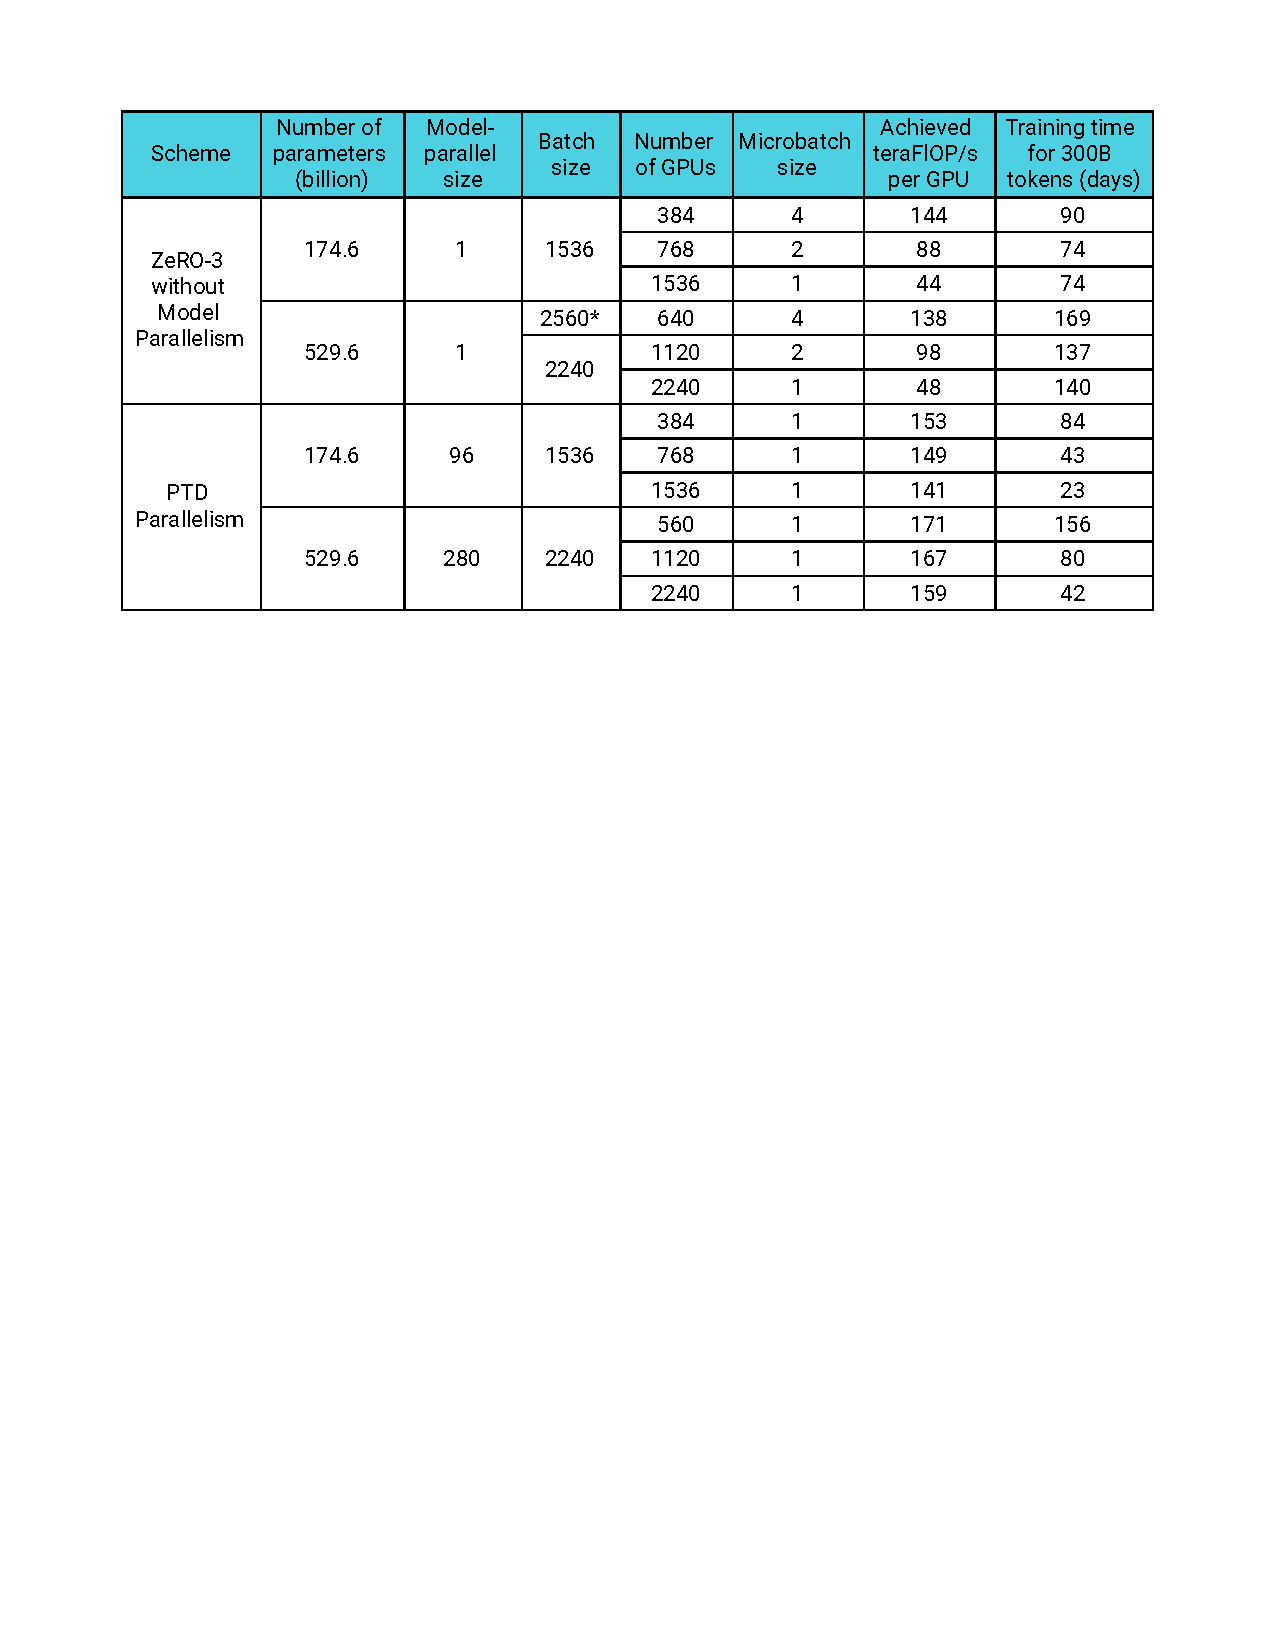
\includegraphics[keepaspectratio=1.0,width=1.65\columnwidth]{figures/zero3_comparison.pdf}
    \vspace{-4.4in}
    \caption{
         Comparison of PTD Parallelism to ZeRO-3 (without model paralllelism). The 530-billion-parameter GPT model did not fit on 560 GPUs when using a microbatch size of 4 with ZeRO-3, so we increased the number of GPUs used to 640 and global batch size to 2560 to provide a throughput estimate (relevant row marked in table with a *).
    }
    \vspace{-0.25in}
    \label{fig:zero3_comparison_table}
\end{table*}

\begin{figure}[t!]
    \centering
    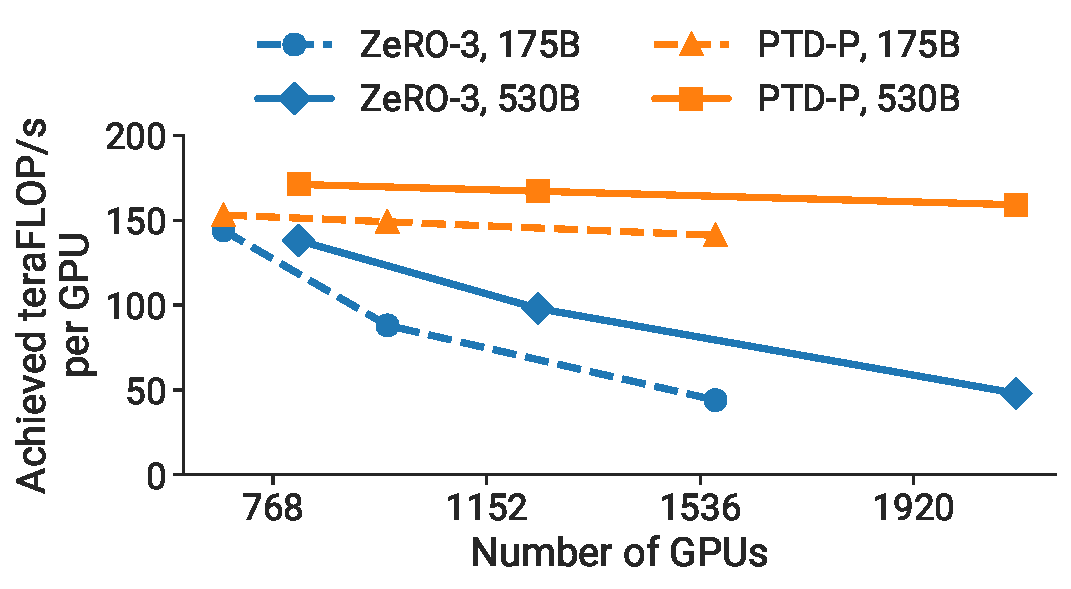
\includegraphics[keepaspectratio=1.0,width=0.9\columnwidth]{figures/zero3_comparison_throughputs.pdf}
    \vspace{-0.05in}
    \caption{
         Throughput per GPU of PTD-P and ZeRO-3 for two different GPT models (the 175B GPT-3 model is shown with dotted lines, and the 530B model is shown with solid lines). Global batch sizes are fixed and ZeRO-3 is used without any model parallelism.
    }
    \label{fig:zero3_comparison_throughputs}
    \vspace{-0.2in}
\end{figure}

\subsection{Comparison to ZeRO-3}

We compare PTD-P to ZeRO-3~\cite{rajbhandari2019zero,rajbhandari2021zero} in Table~\ref{fig:zero3_comparison_table} and Figure~\ref{fig:zero3_comparison_throughputs} for the standard GPT-3 model architecture, as well as the 530-billion-parameter model from Table~\ref{fig:megatron_scaling}. The results provide a point of comparison to a method that does not use model parallelism. We integrated ZeRO into our codebase using the \texttt{DeepSpeed} Python library~\cite{deepspeed}. We keep the global batch size the same as we increase the number of GPUs. With fewer GPUs and a microbatch size of 4, PTD-P results in $6\%$ and $24\%$ higher throughput for the 175- and 530-billion-parameter models respectively. As we increase the number of GPUs, PTD-P scales more gracefully than ZeRO-3 in isolation (see Figure~\ref{fig:zero3_comparison_throughputs}). For example, by doubling the number of GPUs (keeping the batch size the same), PTD-P outperforms ZeRO-3 by $70\%$ for both models due to less cross-node communication. We note that we have only considered ZeRO-3 without tensor parallelism. ZeRO-3 can be combined with model parallelism to potentially improve its scaling behavior.

\subsection{Pipeline Parallelism}
We now evaluate the weak-scaling performance of pipeline parallelism in isolation, and also compare the performance of the non-interleaved schedule to the interleaved schedule.

\subsubsection{Weak Scaling}

\begin{figure}[t!]
    \centering
    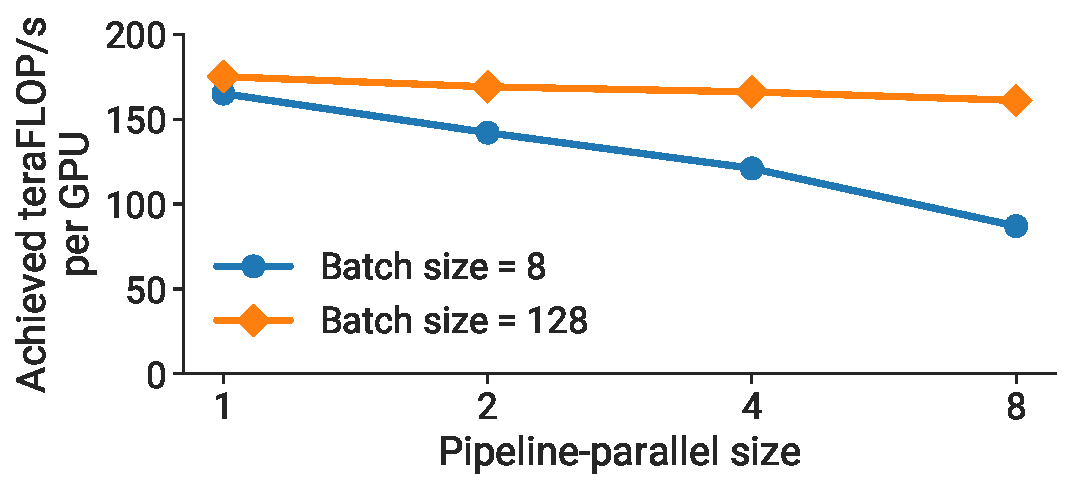
\includegraphics[keepaspectratio=1.0,width=0.9\columnwidth]{figures/pipeline_parallelism_weak_scaling.pdf}
    \vspace{-0.1in}
    \caption{
         Throughput per GPU of pipeline parallelism using two different batch sizes in a weak-scaling experiment setup (model size increases with the pipeline-parallel size).
    }
    \label{fig:pipeline_parallelism_weak_scaling}
    \vspace{-0.1in}
\end{figure}

We evaluate the scaling of the default non-interleaved pipeline-parallel schedule using a weak scaling setup, a GPT model with 128 attention heads and a hidden size of 20480, and a microbatch size of 1. As we increase the number of pipeline stages, we also increase the size of the model by proportionally increasing the number of layers in the model, e.g., with a pipeline-parallel size of 1, we use a model with 3 transformer layers and ~15 billion parameters, and with a pipeline-parallel size of 8, we use a model with 24 transformer layers and ~121 billion parameters. We use a tensor-parallel size of 8 for all configurations, and vary the total number of A100 GPUs used from 8 to 64. Figure~\ref{fig:pipeline_parallelism_weak_scaling} shows throughput per GPU for two different batch sizes to illustrate the impact of the pipeline bubble, which behaves as $\frac{p-1}{m}$ (\S\ref{sec:pipeline_parallelism_bubble}). As expected, the higher batch size scales better since the pipeline bubble is amortized over more microbatches.

\subsubsection{Interleaved versus Non-Interleaved Schedule}

\begin{figure}[t!]
    \centering
    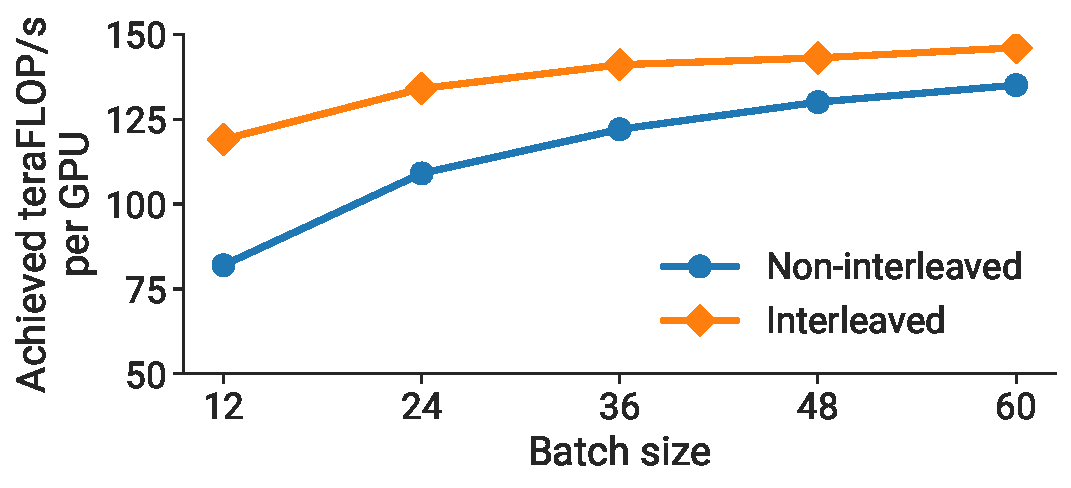
\includegraphics[keepaspectratio=1.0,width=0.9\columnwidth]{figures/gpt_175b_interleaved_vs_default.pdf}
    \vspace{-0.1in}
    \caption{
         Throughput per GPU of interleaved and non-interleaved schedules for a GPT model (175 billion parameters) on 96 GPUs.
    }
    \vspace{-0.1in}
    \label{fig:interleaved_vs_default}
\end{figure}

Figure~\ref{fig:interleaved_vs_default} shows the per-GPU-throughput for interleaved and non-interleaved schedules on the GPT-3~\cite{gpt3} model with
175 billion parameters (96 layers, 96 attention heads, hidden size of 12288).
The interleaved schedule with the scatter/gather communication optimization has higher computational performance than the non-interleaved (default) schedule. This gap closes as the batch size increases due to two reasons: (a) as the batch size increases, the bubble size in the default schedule decreases, and (b) the amount of point-to-point communication within the pipeline is proportional to the batch size, and consequently the non-interleaved schedule catches up as the amount of communication increases (the interleaved schedule features more communication per sample). Without the scatter/gather optimization, the default schedule performs better than the interleaved schedule at larger batch sizes (not shown).

\subsection{Comparison of Parallel Configurations}
\label{sec:evaluation_parallel_configurations}

In this sub-section, we show the various tradeoffs associated with combining different parallelization dimensions. In particular, we show the performance for parallel configurations using the same number of GPUs for a given model and multiple batch sizes.

\subsubsection{Tensor versus Pipeline Parallelism}

\begin{figure}[t!]
    \centering
    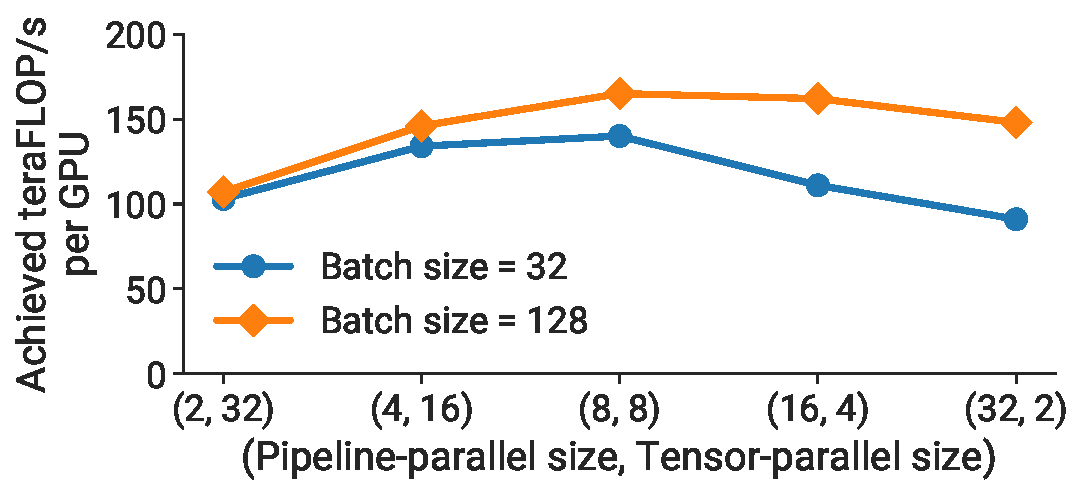
\includegraphics[keepaspectratio=1.0,width=0.9\columnwidth]{figures/pipeline_and_tensor_model_parallelism.pdf}
    \vspace{-0.1in}
    \caption{
         Throughput per GPU of various parallel configurations that combine pipeline and tensor model parallelism using a GPT model with 162.2 billion parameters and 64 A100 GPUs.
    }
    \vspace{-0.1in}
    \label{fig:pipeline_and_tensor_model_parallelism}
\end{figure}

\begin{figure}[t!]
    \centering
    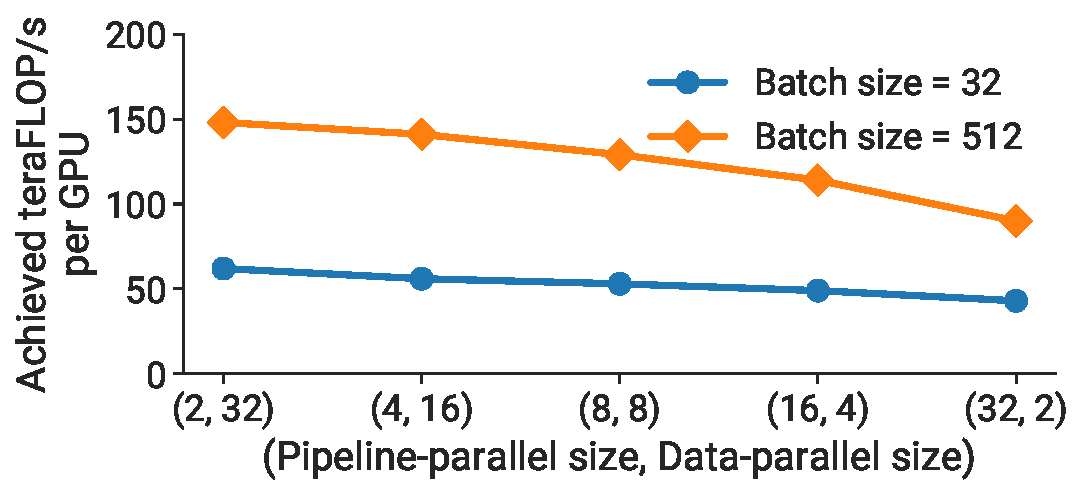
\includegraphics[keepaspectratio=1.0,width=0.9\columnwidth]{figures/data_and_pipeline_model_parallelism.pdf}
    \vspace{-0.1in}
    \caption{
         Throughput per GPU of various parallel configurations that combine data and pipeline model parallelism using a GPT model with 5.9 billion parameters, three different batch sizes, microbatch size of 1, and 64 A100 GPUs.
    }
    \vspace{-0.1in}
    \label{fig:data_and_pipeline_model_parallelism}
\end{figure}

\begin{figure}[t!]
    \centering
    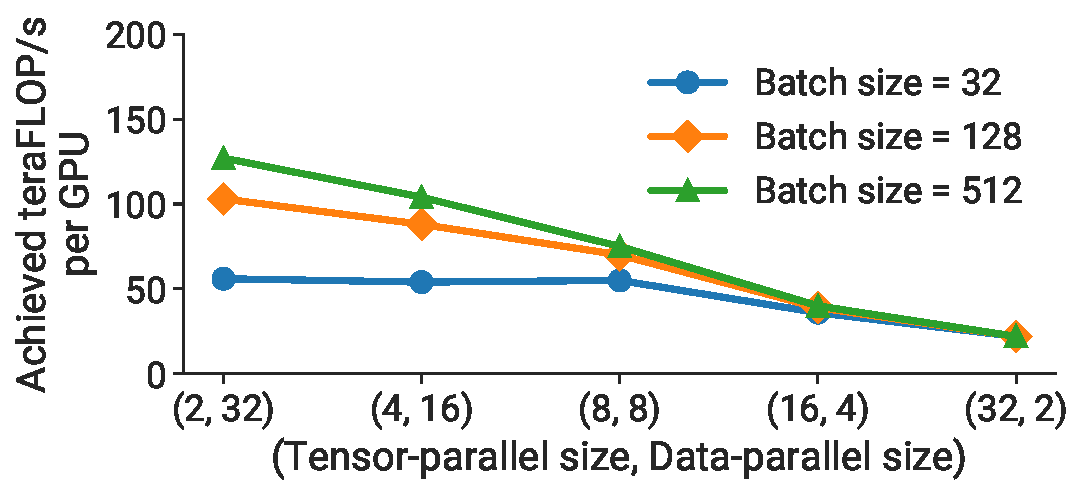
\includegraphics[keepaspectratio=1.0,width=0.9\columnwidth]{figures/data_and_tensor_model_parallelism.pdf}
    \vspace{-0.1in}
    \caption{
         Throughput per GPU of various parallel configurations that combine data and tensor model parallelism using a GPT model with 5.9 billion parameters, three different batch sizes, microbatch size of 1, and 64 A100 GPUs.
    }
    \vspace{-0.1in}
    \label{fig:data_and_tensor_model_parallelism}
\end{figure}

\begin{figure}[t!]
    \centering
    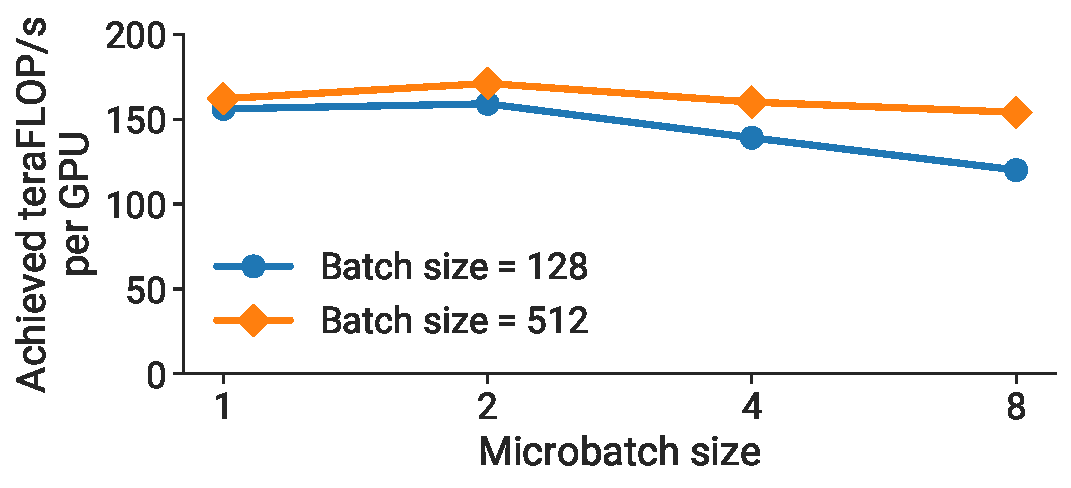
\includegraphics[keepaspectratio=1.0,width=0.9\columnwidth]{figures/microbatch_size_91B.pdf}
    \vspace{-0.1in}
    \caption{
         Throughput per GPU of a $(t, p) = (8, 8)$ parallel configuration for different microbatch sizes on a GPT model with 91 billion parameters, for two different batch sizes using 64 A100 GPUs.
    }
    \vspace{-0.1in}
    \label{fig:microbatch_size}
\end{figure}

We evaluate the impact of pipeline and tensor model parallelism on performance for a given model and batch size. The empirical results in Figure~\ref{fig:pipeline_and_tensor_model_parallelism} show the importance of using both tensor and pipeline model parallelism in conjunction to train a 161-billion-parameter GPT model (32 transformer layers to support pipeline-parallel size of 32, 128 attention heads, hidden size of 20480) with low communication overhead and high compute resource utilization. We observe that tensor model parallelism is best within a node (DGX A100 server) due to its expensive all-reduce communication. Pipeline model parallelism, on the other hand, uses much cheaper point-to-point communication that can be performed across nodes without bottlenecking the entire computation. However, with pipeline parallelism, significant time can be spent in the pipeline bubble: the total number of pipeline stages should thus be limited so that the number of microbatches in the pipeline is a reasonable multiple of the number of pipeline stages. Consequently, we see peak performance when the tensor-parallel size is equal to the number of GPUs in a single node (8 with DGX A100 nodes). This result indicates that neither tensor model parallelism (used by Megatron~\cite{shoeybi2019megatron}) nor pipeline model parallelism (used by PipeDream~\cite{narayanan2021memory} and others) in isolation can match the performance of using both techniques in conjunction.

\subsubsection{Pipeline versus Data Parallelism}

We evaluate the impact of data and pipeline model parallelism on performance for a GPT model with 5.9 billion parameters (32 transformer layers, 32 attention heads, hidden size of 3840) in Figure~\ref{fig:data_and_pipeline_model_parallelism}. We use a smaller model than before since we want to show performance for models that fit when the model-parallel size is only 2. For simplicity, we keep the microbatch size equal to 1 in these experiments. We see that for each batch size, the throughput decreases as the pipeline-parallel size increases, matching our analytical model from \S\ref{sec:data_and_model_parallelism_analytical_model}. Pipeline model parallelism should be used primarily to support the training of large models that do not fit on a single worker, and data parallelism should be used to scale up training.

\subsubsection{Tensor versus Data Parallelism}

We also evaluate the impact of data and tensor model parallelism on performance for the same GPT model with 5.9 billion parameters in Figure~\ref{fig:data_and_tensor_model_parallelism} (smaller model used for same reason as above). As before, we keep the microbatch size equal to 1 initially. With larger batch sizes and a microbatch size of 1, data-parallel communication is infrequent; the all-to-all communication required in tensor model parallelism needs to be performed for \emph{every} microbatch in a batch. This all-to-all communication with tensor model parallelism dominates end-to-end training time, especially when communication needs to be performed across multi-GPU nodes. Additionally, as the tensor-model-parallel size increases, we perform smaller matrix multiplications on every GPU, decreasing utilization on each GPU.

\vspace{0.1in}
We should note that although data parallelism can lead to efficient scaling, we cannot use data parallelism in isolation for very large models with a limited training batch size because of a) insufficient memory capacity, and b) scaling limitations of data parallelism (e.g., GPT-3 was trained to convergence with a batch size of $1536$. Data parallelism thus supports parallelization to only $1536$ GPUs; however, roughly $10,000$ GPUs were used to train this model in a reasonable amount of time).

\subsection{Microbatch Size}

We evaluate the impact of the microbatch size on the performance of parallel configurations that combine pipeline and tensor model parallelism in Figure~\ref{fig:microbatch_size} for a model with 91 billion parameters ($(t, p) = (8, 8)$). We see that the best microbatch size is 2 for this model; the optimal microbatch size is different for other models (not shown in Figure) and \emph{model-dependent}. For a given batch size, increasing the microbatch size decreases the number of microbatches in the pipeline ($m$), leading to a larger pipeline bubble; however, increasing the microbatch size can also improve GPU utilization by increasing the arithmetic intensity of executed kernels. These two factors are at odds with each other, which makes the choice of optimal microbatch size challenging. Our analytical model from \S\ref{sec:data_and_model_parallelism_analytical_model} reasonably approximates true performance, and can be used as a proxy to determine how to pick this hyperparameter value for various training configurations and models.

\begin{figure}[t!]
    \centering
    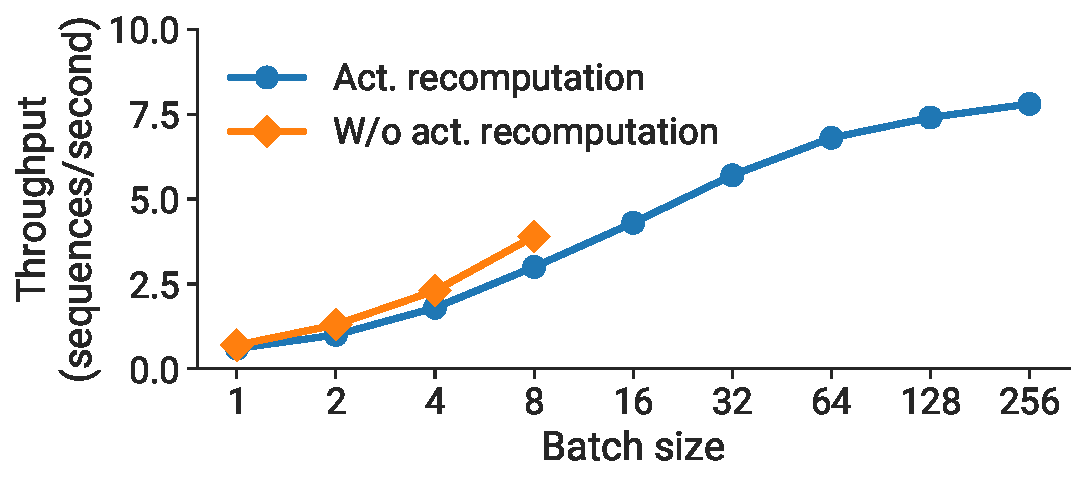
\includegraphics[keepaspectratio=1.0,width=0.9\columnwidth]{figures/gpt_145b_activation_recomputation.pdf}
    \vspace{-0.1in}
    \caption{
         Throughput (in sequences per second) with and without activation recomputation for a GPT model with 145 billion parameters using 128 A100 GPUs ($(t, p) = (8, 16)$).
    }
    \vspace{-0.1in}
    \label{fig:activation_recomputation}
\end{figure}

\subsection{Activation Recomputation}

Figure~\ref{fig:activation_recomputation} shows throughput with and without activation recomputation for a GPT model with 145 billion parameters (80 transformer layers, 96 attention heads, hidden size of 12288) using 128 A100 GPUs, $(t, p) = (8, 16)$, and a range of batch sizes. For small batch sizes, activation recomputation leads to up to $33\%$ lower throughput (in sequences per second) due to the extra forward pass that needs to be executed during the backward pass. However, activation recomputation is needed to support larger batch sizes. Throughput at large batch sizes with activation recomputation is up to $2\times$ higher than the best throughput achieved without activation recomputation (for a smaller batch size) due to a smaller pipeline bubble.

\begin{figure}[t!]
    \centering
    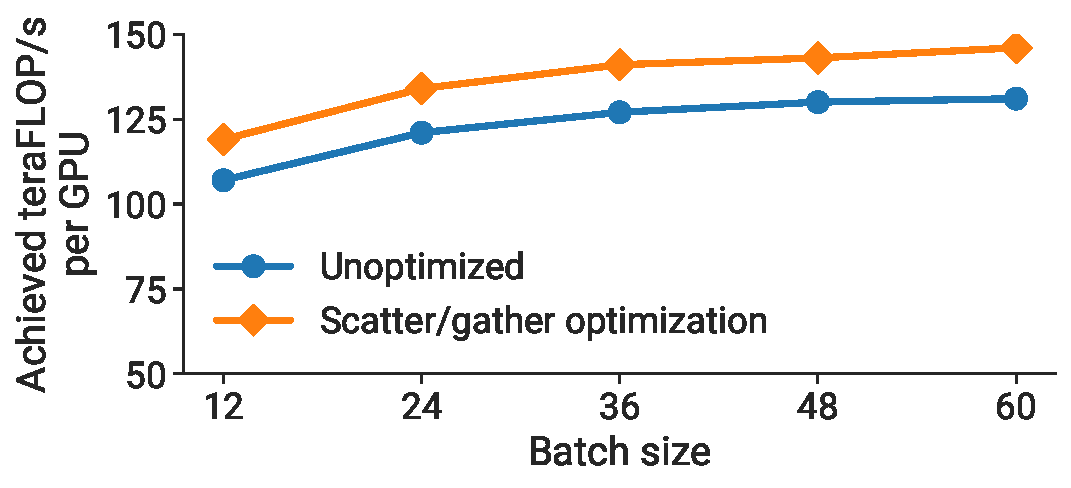
\includegraphics[keepaspectratio=1.0,width=0.9\columnwidth]{figures/gpt_175b_scatter_gather_optimization.pdf}
    \vspace{-0.1in}
    \caption{
         Throughput per GPU with and without the scatter/gather optimization for a GPT model with 175 billion parameters using 96 A100 GPUs and the interleaved schedule.
    }
    \vspace{-0.1in}
    \label{fig:scatter_gather_optimization_eval}
\end{figure}

\subsection{Scatter-Gather Optimization}

Figure~\ref{fig:scatter_gather_optimization_eval} shows per-GPU-throughput with and without (unoptimized) the scatter/gather communication optimization for the GPT-3 model with 175 billion parameters. We see an improvement of up to 11\% in throughput for communication-intensive schedules (large batch size with interleaving) by reducing the amount of communication over cross-node links.

\subsection{Fused Operators}
We also evaluate the performance impact of operator fusion described in \S\ref{sec:computation_optimizations}. For the GPT-3 model (175 billion parameters), throughput increased by 19\% with fusion (113 teraFLOP/s per GPU to 135 teraFLOP/s per GPU). For the larger GPT model with 530 billion parameters (model configuration in Figure~\ref{fig:megatron_scaling}), throughput increased by 11\% (133 teraFLOP/s per GPU to 148 teraFLOP/s per GPU).


\subsection{Inter-Node Communication Bandwidth}
Our strong results are a byproduct of using an optimized software and hardware stack \emph{together}. In particular, we take advantage of the high-bandwidth communication links between GPUs on the same server and across servers. On the trillion-parameter model with 3072 GPUs, we observed that the effective bisection bandwidth of point-to-point communication among pipeline stages is 892 GB/s, while the effective bisection bandwidth of all-reduce operations among data-parallel replicas is 12.9 TB/s. A less-optimized partitioning of operators across devices would lead to more inter-node communication, hampering scaling performance.


\subsection{Checkpoint Loading and Saving}

An important practical consideration for the training of large models is loading and saving model checkpoints, which are especially large for the models considered in this paper. For example, the trillion-parameter model has a checkpoint of size 13.8 terabytes. The initial load of checkpoints for the trillion-parameter model by all 384 nodes (3072 GPUs) reaches a peak read bandwidth of 1TB/s, the maximum read throughput possible from the parallel filesystem. Checkpoint saves reach 40\% of peak write bandwidth (273 GB/s).